\chapter{BIT 2019 Flight Hardware Integration}
\section{Overview}
Before SuperBIT can can collect scientific data it must fly. 
\par
In this section I give a brief summary of my personal contributions to the hardware integration efforts for the upcoming 2019 flight. 

\section{UFO System}
Talk about why we need UFOs what I did for them (the circuit) and add an image. also programming the UFO.

\section{Computer \& Electronic Upgrades}
Talk about MCC replacing freeform with Mesa fpga and what mesa does. 
Talk about IFC replacing the computer with new one, removing the serial and going with USB instead and putting in mesa and programming it.

\begin{figure}
    \begin{small}
        \begin{center}
            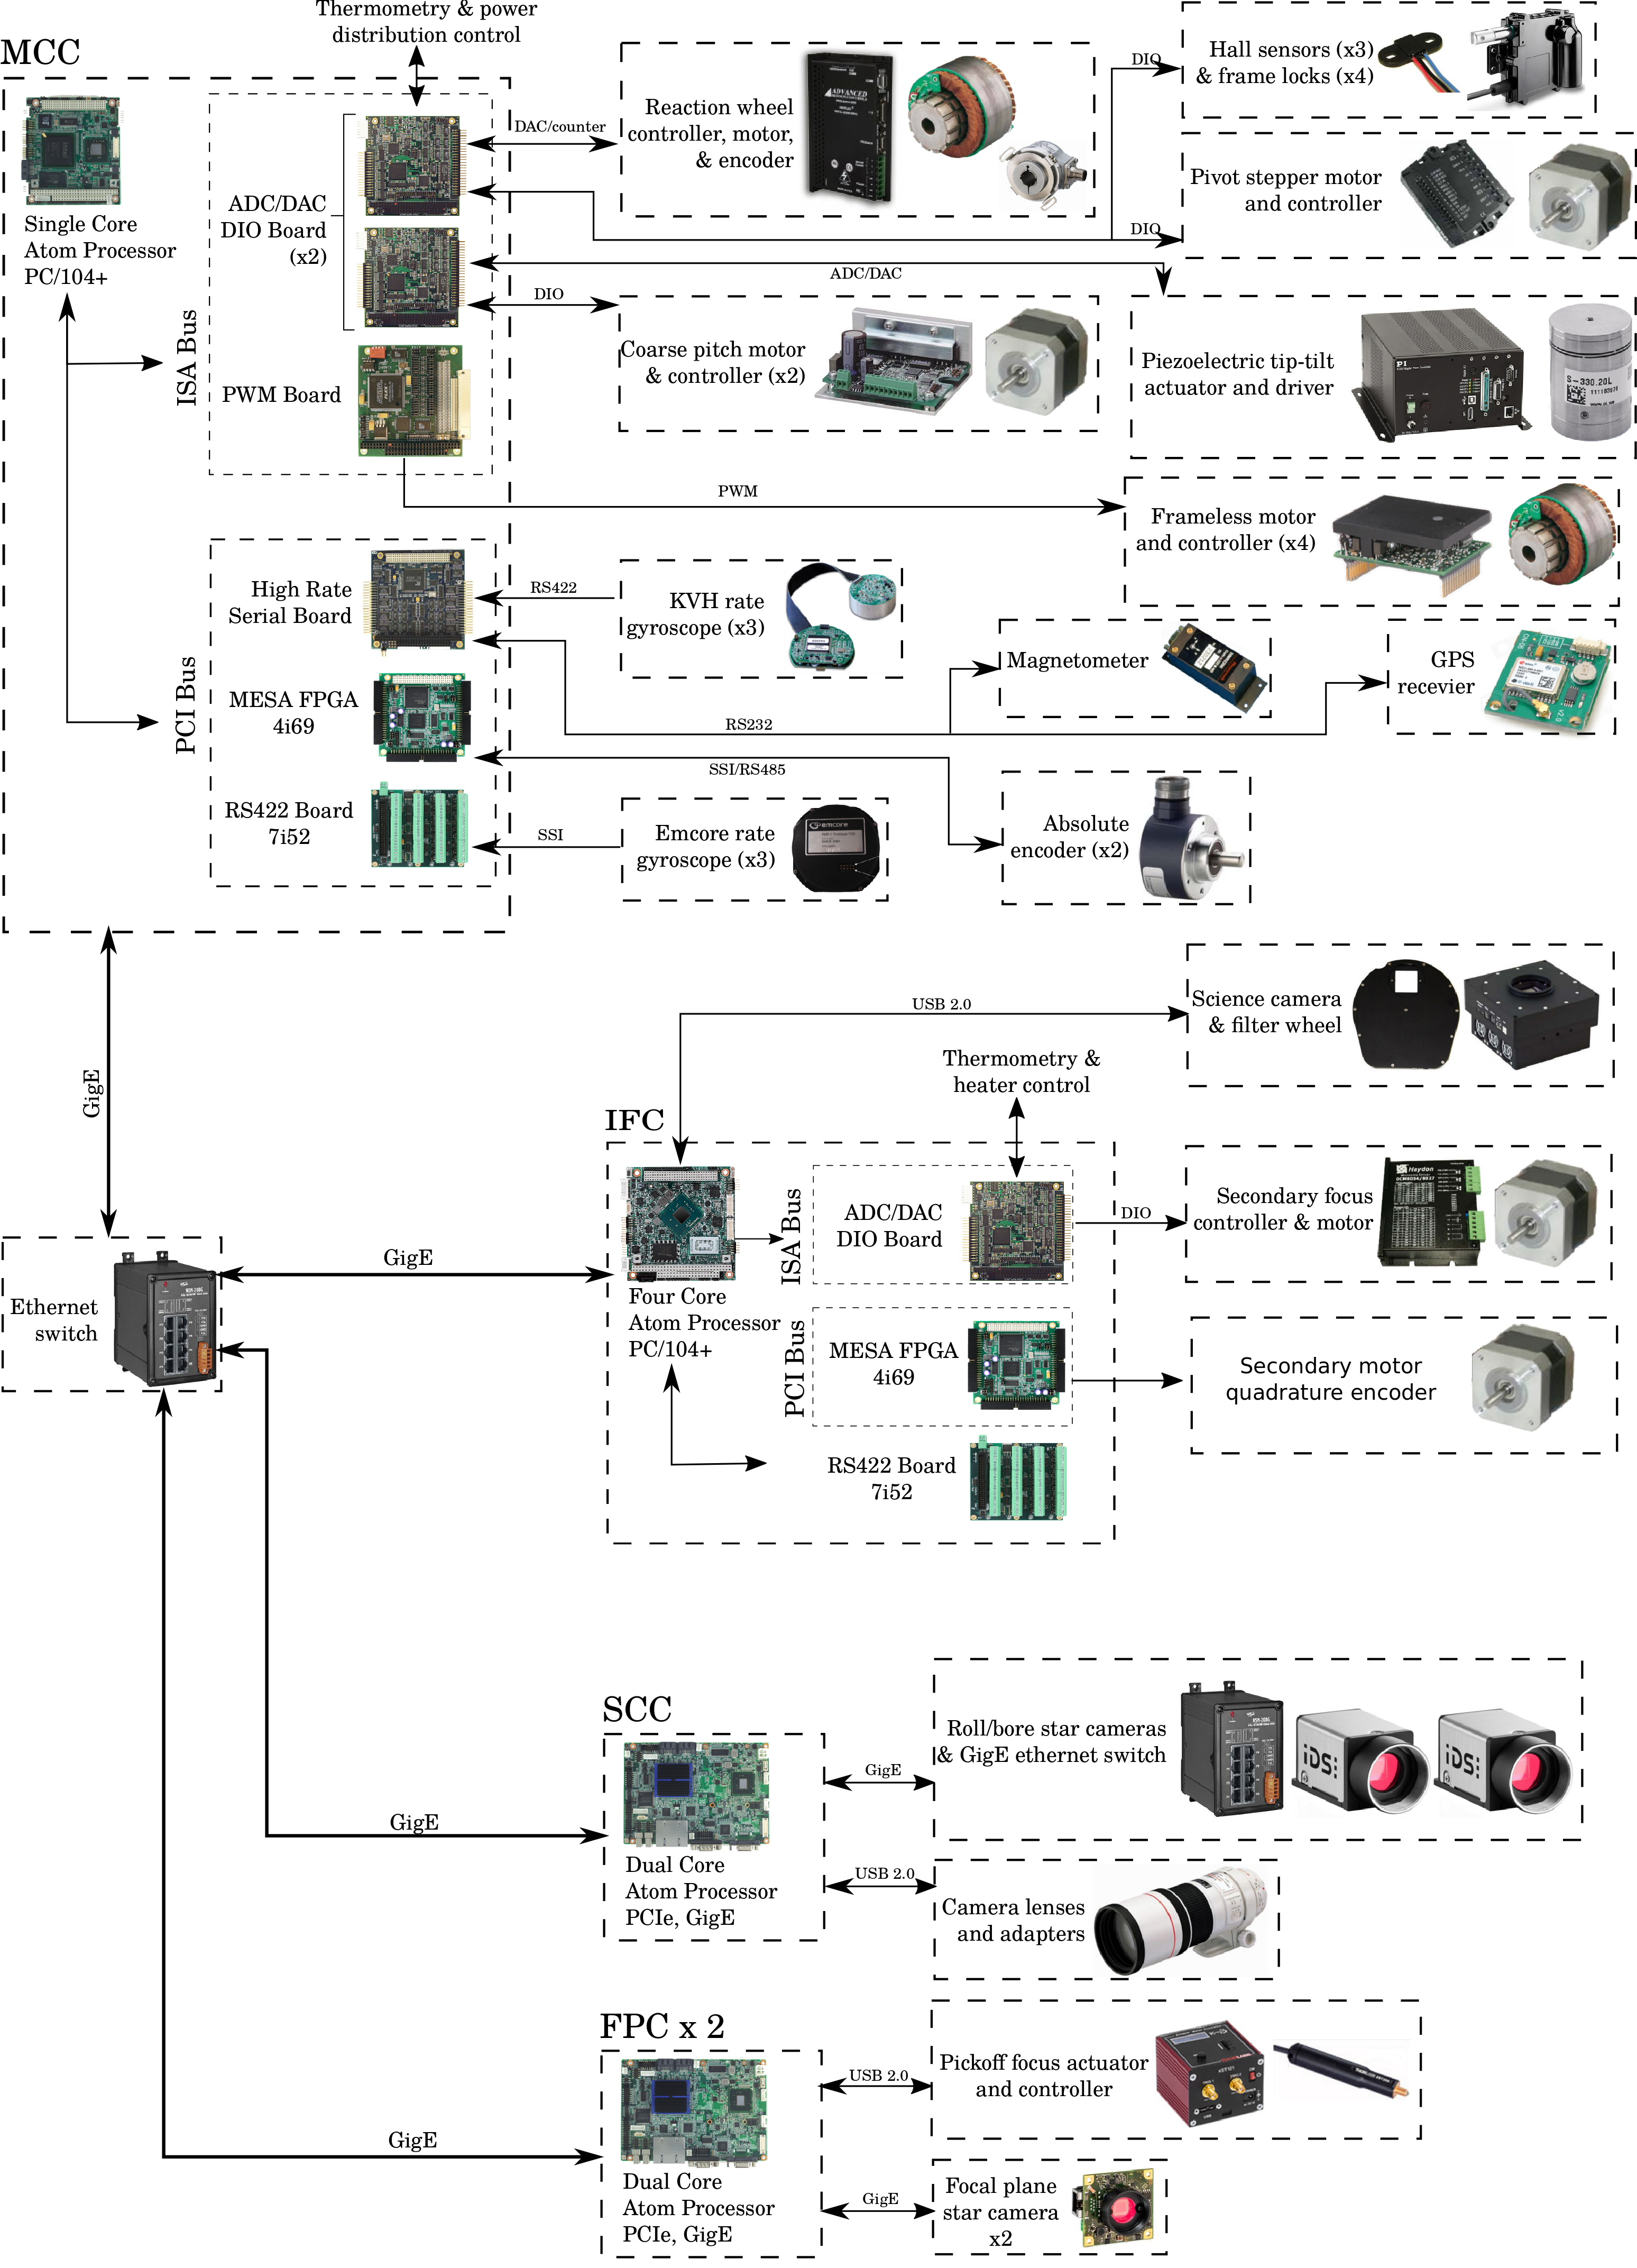
\includegraphics[width=0.95\textwidth]{Hardware/figs/electronics.png}
        \end{center}
        \caption{BIT computer and electronics layout for 2019 flight.}
        \label{fig:electronics}
    \end{small}
\end{figure}


\section{Secondary Motors}
characterize them from ajays notes. and from my code work

\section{Baffle Mounting Device}
why do we need it what is mount on it why did it need sorbathane and thermal calcs.

\section{Battery Boxes}
why do we need them what do they do and how do they operate.

\section{Inner Frame Design}


